\section{Results}\label{sec:completed_comparison_results}

We evaluate the performance of the proposed control and of impedance control by
subjecting the amputee model to terrains that are flat for \unit[10]{meters} and
then feature steps drawn from uniform distributions for another
\unit[90]{meters}.  The widths of the distributions are constant but vary among
the terrains to test the control performance on steps of increasing steepness
(\unit[0]{cm} to $\pm \unit[14]{cm}$, \unit[2]{cm} increments, total of 8
terrains). 

\begin{figure}[t]
    \centering
    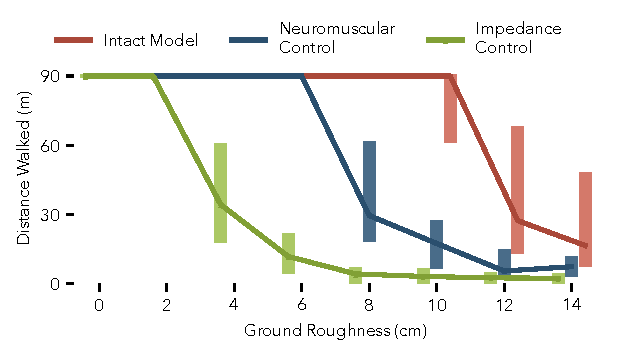
\includegraphics[width = \columnwidth]{distsWalked}
    \caption{Control performance of simulated prosthesis on rough terrain. The
    distances walked over terrains with different ground roughness are compared
    between the amputee model using a powered knee-ankle prosthesis with
    impedance control (green) and hybrid neuromuscular control (blue) as well
    as with the unimpaired human model (red). Shown are the median and range
    ($25^\textrm{th}$ and $75^\textrm{th}$ percentiles) of the covered
    distances for 50 terrains sampled at each roughness level.
    }\label{fig:distsWalked}
\end{figure}
\Cref{fig:distsWalked} shows the distances the amputee model walks over 50
trials at each roughness level (proposed neuromuscular control in blue,
impedance control in green). Most of the trials with the impedance-controlled
prosthesis cover the full distance up to a roughness of \unit[2]{cm}. At a
roughness of \unit[4]{cm}, however, the median distance drops to \unit[34]{m},
which further declines as the roughness increases. In contrast, the  prosthesis
using the neuromuscular control, allows the amputee model to walk the full
distance up to a roughness of \unit[6]{cm}. Moreover, neuromuscular control has
a similar distribution of distances walked at a roughness of \unit[8]{cm} as
impedance control has at a roughness of \unit[4]{cm}.

Although the prosthesis using neuromuscular control significantly improves the
robustness of the amputee model on rough terrain, the performance trails by a
large margin that of an unimpaired model (\cref{fig:distsWalked}, red line), for
which most of the trials covered the full distance up to a roughness of
\unit[10]{cm}.  Limiting the swing leg placement targets in the neuromuscular
prosthesis control to constant angles may account for some of this performance
gap. In future work, we may overcome this limitation by estimating the amputee's
center of mass velocity and stance ankle position so that the prosthesis control
can take advantage of the full leg placement policy (\cref{eq:simbicon}). Other
sources for the performance gap could stem from differences in the inertial
properties between the prosthesis and the healthy leg, delay and inaccuracy in
the series elastic actuator torque tracking, and the increased number of
parameters in the asymmetric amputee model, which can reduce the quality of the
optimized solutions.

A possible explanation for why the neuromuscular control produces more robust
behavior than impedance control is the former's attempt to mimic the underlying
dynamics and goals of human motor control rather than to track impedance
behavior about a predefined motion for each individual joint. To illustrate this
difference, we subject the amputee model with both control strategies to a
simulated trip in the form of a $\unit[15]{N \cdot s}$ impulse applied at 5\% of
the undisturbed swing duration. 

\begin{figure*}[t]
    \centering
    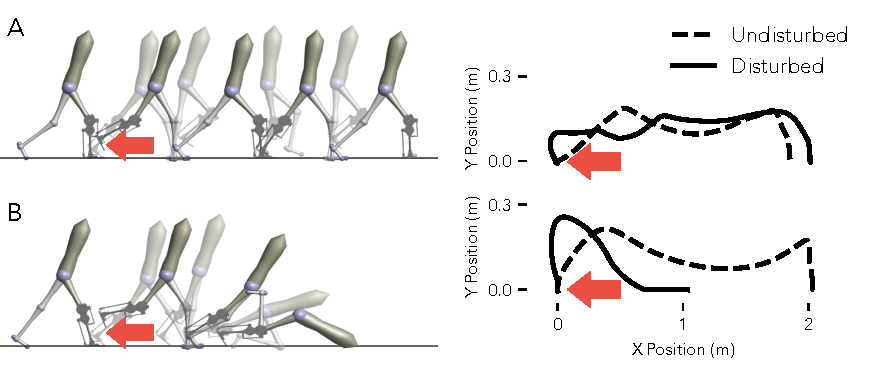
\includegraphics{impulseResponseAnnotated}
    \caption{Tripping response of the amputee model with neuromuscular (A) and
    impedance control (B) of the prosthesis. Shown are the prosthetic toe
    trajectories during undisturbed gait (dashed line) and when disturbed by a
    $\unit[15]{N \cdot s}$ impulse (solid line). The neuromuscular controller
    effectively responds to the disturbance and maintains a qualitatively
    similar toe trajectory. The impedance controller leads to foot scuffing and
    an eventual fall.
    }\label{fig:ImpulseResponses}
\end{figure*}

\Cref{fig:ImpulseResponses}A shows the toe trajectory of the prosthesis using
neuromuscular control both in the undisturbed and disturbed cases. While the
impulse causes a large deviation from the nominal trajectory in early swing, the
controller quickly recovers. From mid-swing onward, the foot follows a
qualitatively similar path, maintains adequate ground clearance, and
successfully reaches a similar foot placement as in the undisturbed case. In
contrast, the prosthesis with impedance control does not respond adequately when
subjected to the disturbance (\cref{fig:ImpulseResponses}B). This is illustrated
by the prosthesis behavior in mid swing, during which it does not react
appropriately to maintain ground clearance of the toe. Rather, the joint-based
impedance functions drive the knee into extension prematurely, and the
prosthetic foot scuffs the ground resulting in a trip and subsequent fall.
